\documentclass[12pt]{article}
\usepackage{latexsym,graphicx}
\usepackage{amssymb}
\usepackage{amsmath} % Added for better math environments
\usepackage{tikz}
\usetikzlibrary{positioning,shapes.gates.logic.US}
\voffset=-.8cm
\hoffset=-1.5cm
\setlength{\textheight}{23cm}
\setlength{\textwidth}{16cm}
\pagestyle{myheadings}
\newtheorem{q} {Q}
\newcommand{\beq}{\begin{q}\hskip.01cm)\hskip.03cm}
\newcommand{\eeq}{\end{q}\newpage}
\newcommand{\df}{\displaystyle\frac}
\newcommand{\dar}{\downarrow}
\newcommand{\ra}{\rightarrow}
\newcommand{\lra}{\leftrightarrow}
\markright {Dr. Petrescu CCP MATH163 Practice Exam 1}
\begin{document}
{\bf Practice Exam 1 Discrete Mathematics 1 } \vskip0.2cm
\vskip.1cm{\bf This is a mandatory homework. Show all your work to get credit. } \vskip0.2cm
{\bf Name}: Valen Li {\bf Due Date}: {\underline{10/03/25}} \vskip.5cm
%%questions \eeq

\beq The following sign is at the entrance of a restaurant: ``No shoes, no shirt, no service." Write this sentence as a conditional proposition. \\

-Lets set p equal to ``The user wears shoes'', q equal to ``The user wears a shirt'', and r equal to ``Service is provided''.
Then $\lnot p$ is ``No shoes'', $\lnot q$ is ``No shirt'', and $\lnot r$ is ``No service''.
The requirement for service is (shoes $\land$ shirt). The conditional proposition is:
$$(\lnot p \land \lnot q) \ra \lnot r$$
\eeq

\beq Write these system specifications in symbols using the propositions:\\v: ``The user enters a valid password,"\\a: ``Access is granted to the user,"\\c: ``The user has contacted the network administrator,"\\and logical connectives. Then determine if the system specifications are consistent (i.e. all 3 statements can be simultaneously true).\\(i) ``The user has contacted the network administrator, but does not enter a valid password."\\(ii) ``Access is granted whenever the user has contacted the network administrator or enters a valid password."\\(iii) ``Access is denied if the user has not entered a valid password or has not contacted the network administrator." \\

i) $C \land \lnot V$ \\

ii) $(C \lor V) \ra A$ \\

iii) $(\lnot V \lor \lnot C) \ra \lnot A$ \\

1.For (i) to be True, we must have $C = \mathbf{T}$ and $V = \mathbf{F}$.
2.Substitute $C=T$ and $V=F$ into (iii):
$$(\lnot F \lor \lnot T) \ra \lnot A \equiv (T \lor F) \ra \lnot A \equiv T \ra \lnot A$$
For (iii) to be True, the conclusion $\lnot A$ must be True, so $A = \mathbf{F}$.
3.Now, check if the truth assignment $V=F, A=F, C=T$ satisfies (ii):
$$(C \lor V) \ra A \equiv (T \lor F) \ra F \equiv T \ra F$$
The statement $T \ra F$ is False.

Since the requirement for (i) and (iii) to be true ($V=F, A=F, C=T$) makes (ii) false, there is no assignment that makes all three true. Therefore, the system specifications are inconsistent.
\eeq

\beq Solve this puzzle: You meet two people, A and B. Each person either always tells the truth or always lies. Person A tells you, ``We are not both truthtellers.''\\Determine, if possible, which type of person each one is. \\

Let $P_A$ be the proposition ``A is a truthteller'' and $P_B$ be the proposition ``B is a truthteller''.
A's statement $S$ is $\lnot (P_A \land P_B)$.

1.Assume A is a Liar ($\lnot P_A$): A's statement $S$ must be False.
$$\lnot S \equiv P_A \land P_B$$
For $P_A \land P_B$ to be True, $P_A$ must be True.
This contradicts our assumption that A is a Liar ($\lnot P_A$). Thus, this case is impossible.

2.Assume A is a Truthteller ($P_A$): A's statement $S$ must be True.
$$S \equiv \lnot (P_A \land P_B)$$
Since $P_A$ is True, $S \equiv \lnot (T \land P_B) \equiv \lnot P_B$.
Since $S$ must be True, $\lnot P_B$ must be True. This means $P_B$ is False.

Conclusion: A must be a truthteller (Knight) and B must be a liar (Knave).
\eeq

\beq Write the following statement and its negation symbolically: "If it is Thursday, then we are going to swim only if it is not raining".\\

Let $p$: ``It is Thursday'', $q$: ``We are going to swim'', $r$: ``It is raining''.
The phrase ``A only if B'' means $A \ra B$. So, ``we are going to swim only if it is not raining'' is $q \ra \lnot r$.
The entire statement is in the form ``If $p$, then $q \ra \lnot r$'':
$$\text{Statement: } p \ra (q \ra \lnot r)$$

To find the negation, we first simplify the statement using logical equivalences:
$$p \ra (q \ra \lnot r) \equiv p \ra (\lnot q \lor \lnot r) \equiv \lnot p \lor (\lnot q \lor \lnot r) \equiv \lnot (p \land q \land r)$$
Now negate the simplified form:
$$\text{Negation: } \lnot (\lnot (p \land q \land r)) \equiv p \land q \land r$$
In English, the negation is: \``It is Thursday, and we are going to swim, and it is raining.''
\eeq

\beq Prove that $ p \rightarrow (q \lor r ) \equiv (p\land \lnot q) \rightarrow r $ by using a series of logical equivalences.\\

$$\begin{array}{rcll}
(p\land \lnot q) \rightarrow r & \equiv & \lnot(p\land \lnot q) \lor r & (\text{Implication Law: } A \ra B \equiv \lnot A \lor B) \\
& \equiv & (\lnot p \lor \lnot(\lnot q)) \lor r & (\text{De Morgan's Law}) \\
& \equiv & (\lnot p \lor q) \lor r & (\text{Double Negation}) \\
& \equiv & \lnot p \lor (q \lor r) & (\text{Associative Law}) \\
& \equiv & p \rightarrow (q \lor r) & (\text{Implication Law})
\end{array}$$
The two expressions are equivalent.
\eeq

\beq Consider this sentence, which is Section 2 of Article I of the U. S. Constitution: \\``No person shall be a Representative who shall not have attained the age of twenty-five years, and been seven years a citizen of the United States, and who shall not, when elected, be an inhabitant of that state in which he shall be chosen."\\(a) Rewrite the sentence in English in the form ``If . . . , then . . . ". \\(b) Using the predicates A(x): ``x is at least twenty-five years old," C(x): ``x has been a citizen of the United States for at least seven years," I(x): ``x, when elected, is an inhabitant of the state in which he is chosen," and R(x): ``x can be a Representative," where the universe for x in all four predicates consists of all people, rewrite the sentence using quantifiers and these predicates. [Note: At the time at which the U. S. Constitution was ratified, the universe for x consisted of landowning males.]\\

a) If a person is a Representative, then that person is at least 25 years old, has been a citizen of the United States for at least 7 years, and is an inhabitant of the state from which they are chosen when elected.\\

b) The sentence establishes the necessary conditions for being a Representative. The form is $R(x) \ra (\text{requirements})$.
$$\forall x (R(x) \rightarrow (A(x) \land C(x) \land I(x)))$$
\eeq

\beq Suppose that the universe for x and y is $\{1,2,3\}$. Also, assume that P(x,y) is a predicate that is true in the following cases, and false otherwise: P(1,3),P(2,1),P(2,2),P(3,1),P(3,2),P(3,3). Determine whether each of the following is true or false:\\(a) $\forall y\exists x (x\neq y \wedge P (x, y))$.\\(b) $\forall x\exists y (x\neq y \wedge \neg P (x, y))$.\\(c) $\forall y\exists x (x\neq y \wedge \neg P (x, y))$.\\

The false cases $\neg P(x,y)$ are: $(1,1), (1,2), (2,3)$.

a) $\forall y\exists x (x\neq y \wedge P (x, y))$. (True)
\begin{itemize}
\item $y=1$: $\exists x \neq 1$ $|$ $P(x, 1)$? Yes, $P(2,1)$ and $P(3,1)$ are True.
\item $y=2$: $\exists x \neq 2$ $|$ $P(x, 2)$? Yes, $P(3,2)$ is True.
\item $y=3$: $\exists x \neq 3$ $|$ $P(x, 3)$? Yes, $P(1,3)$ is True.
\end{itemize}

b) $\forall x\exists y (x\neq y \wedge \neg P (x, y))$. (False)
\begin{itemize}
\item $x=1$: $\exists y \neq 1$ $|$ $\neg P(1, y)$? Yes, $\neg P(1,2)$ is True.
\item $x=2$: $\exists y \neq 2$ $|$ $\neg P(2, y)$? Yes, $\neg P(2,3)$ is True.
\item $x=3$: $\exists y \neq 3$ $|$ $\neg P(3, y)$? No. $P(3,1), P(3,2), P(3,3)$ are all True, so $\neg P(3,y)$ is never True.
\end{itemize}
Since it fails for $x=3$, the statement is False.

c) $\forall y\exists x (x\neq y \wedge \neg P (x, y))$. (False)
\begin{itemize}
\item $y=1$: $\exists x \neq 1$ $|$ $\neg P(x, 1)$? No. $P(1,1)$ is False (so $\neg P(1,1)$ is True, but $x \neq 1$ is required). $P(2,1)$ and $P(3,1)$ are True, so $\neg P(2,1)$ and $\neg P(3,1)$ are False.
\end{itemize}
Since it fails for $y=1$, the statement is False.
\eeq

\beq Determine whether this argument is valid: \\Lynn works part time or full time. ($P \lor F$)\\ If Lynn does not play on the team, then she does not work part time. ($\lnot T \ra \lnot P$)\\If Lynn plays on the team, she is busy. ($T \ra B$)\\Lynn does not work full time. ($\lnot F$)\\Therefore, Lynn is busy. ($\therefore B$) \\

The argument is valid.
$$\begin{array}{rll}
1. & P \lor F & (\text{Premise 1}) \\
2. & \lnot T \ra \lnot P & (\text{Premise 2}) \\
3. & T \ra B & (\text{Premise 3}) \\
4. & \lnot F & (\text{Premise 4}) \\
5. & P & (\text{Disjunctive Syllogism from 1 and 4}) \\
6. & P \ra T & (\text{Contrapositive from 2}) \\
7. & T & (\text{Modus Ponens from 5 and 6}) \\
8. & B & (\text{Modus Ponens from 7 and 3})
\end{array}$$
The conclusion $B$ logically follows from the premises.
\eeq

\beq Give a proof by contradiction of: ``If $n$ is an even integer, then $3n + 7$ is odd."\\

We want to prove $p \ra q$, where $p$: ``$n$ is an even integer'' and $q$: ``$3n + 7$ is odd''.
Assume the negation of the conclusion, $\lnot q$, holds: $3n + 7$ is even.
Since $n$ is an even integer (premise $p$), we can write $n = 2k$ for some integer $k$.
Substituting $n = 2k$ into the assumption:
$$3n + 7 = 3(2k) + 7 = 6k + 7$$
By our assumption, $6k + 7$ is even, so $6k + 7 = 2m$ for some integer $m$.
$$6k + 7 = 2m$$
$$6k - 2m = -7$$
$$2(3k - m) = -7$$
Let $j = 3k - m$. Since $k$ and $m$ are integers, $j$ is an integer.
$$2j = -7$$
This equation states that an even integer $2j$ is equal to an odd integer $-7$. This is a contradiction.
Therefore, our assumption ($\lnot q$) must be false, and the original
conclusion ($q$) that $3n+7$ is odd must be true.
\eeq

\beq Find the output of the following logic gate:\vskip.8cm 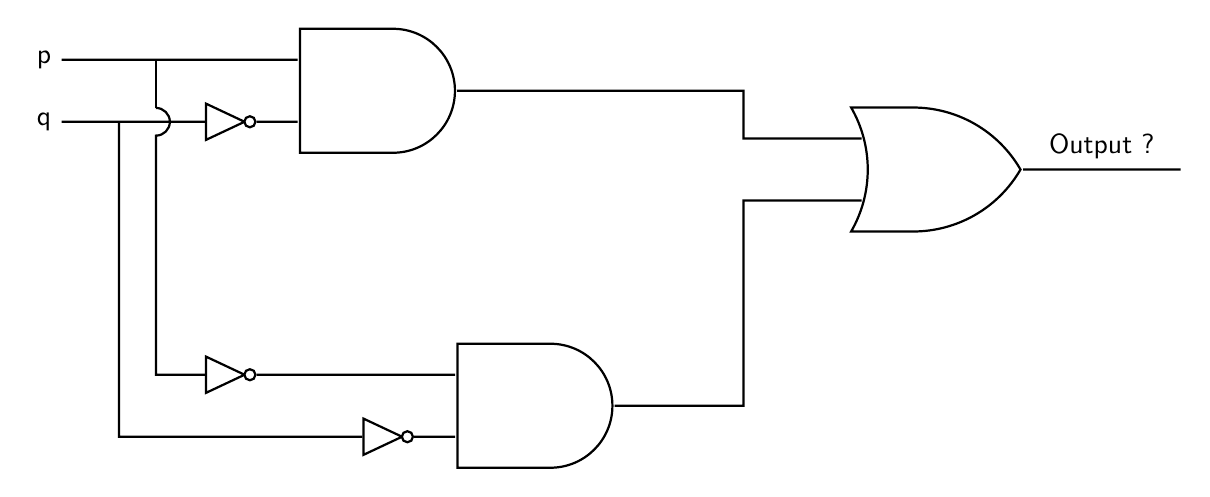
\begin{tikzpicture}[
% you can find documentation here: https://tikz.dev/library-circuits#autosec-5292
        %Environment config
        font=\sffamily,
        thick,
        %Environment styles
        GateCfg/.style={
            logic gate inputs={normal,normal,normal},
            draw,
            scale=2
        }
    ]
    \path
        (0,0) node[and gate US,GateCfg](AND1){} 
            ++ (2,-4) node[and gate US,GateCfg](AND2){} 
            ++ (5,3) node[or gate US,GateCfg](OR1){}
        (AND1.input 3)
            ++ (-1,0) node[not gate US, draw](N1){}
        (AND2.input 3)
            ++ (-1,0) node[not gate US, draw](N2){}
        (AND2.input 1 -| N1)
            node[not gate US, draw](N3){};

    \draw
        (OR1.input 1) -- ++(-1.5,0) |- (AND1.output)
        (OR1.input 3) -- ++(-1.5,0) |- (AND2.output)
        (N2.output)--(AND2.input 3)
        (N1.output)--(AND1.input 3)
        (N3.output)--(AND2.input 1)
        (AND1.input 1) 
            -- ++(-3,0) coordinate (init) node[anchor=east]{p}
            node[pos=0.6](temp){}
        (N1-| temp)
            ++(0,5pt) edge (temp.center)
            arc (90:-90:5pt) |- (N3.input)
        (init |- N1) node[anchor=east]{q} 
            -- (N1.input) node[pos=0.4](temp2){}
        (temp2.center) |- (N2.input)
        (OR1.output) -- ++(2,0) node [midway,anchor=south]{Output ?};
    \end{tikzpicture} 

$$ (p \land \lnot q) \lor (\lnot p \land \lnot q) $$
\eeq

\beq Prove, using whatever method you want, that at least one of the real numbers $a_1, a_2, ..., a_n$ is greater than or equal to the average of these numbers.\\
  

1. Let $\bar{a}$ be the average of the $n$ real numbers $a_1, a_2, \dots, a_n$.
2. By the definition of the average, we have:
$$\bar{a} = \df{a_1 + a_2 + \dots + a_n}{n}$$
3. Multiplying by $n$ gives:
$$n \bar{a} = a_1 + a_2 + \dots + a_n$$
4. Rearranging the terms shows that the sum of the differences between each number and the average is zero:
$$0 = (a_1 - \bar{a}) + (a_2 - \bar{a}) + \dots + (a_n - \bar{a})$$

For a sum of $n$ real numbers to equal zero, it is impossible for all $n$ numbers to be strictly negative. If $(a_i - \bar{a}) < 0$ for all $i$, the sum would be strictly less than zero.

Therefore, at least one of the difference terms, say $(a_k - \bar{a})$, must be greater than or equal to zero:
$$a_k - \bar{a} \geq 0$$
Adding $\bar{a}$ to both sides yields the desired result:
$$a_k \geq \bar{a}$$
We conclude that at least one of the numbers is greater than or equal to the average.
\eeq

\beq Prove by contraposition: $x\in {\mathbb R}, x^2 - 6x+5>0 \rightarrow x\geq 5\; \lor \; x\leq 1$\\

Let $P$ be $x^2 - 6x+5>0$ and $Q$ be $x\geq 5 \lor x\leq 1$. We prove the contrapositive $\lnot Q \rightarrow \lnot P$.
\begin{itemize}
\item Hypothesis ($\lnot Q$): The negation of $x\geq 5 \lor x\leq 1$ is $x < 5 \land x > 1$, or $1 < x < 5$.
\item Conclusion ($\lnot P$): The negation of $x^2 - 6x+5>0$ is $x^2 - 6x+5 \leq 0$.
\end{itemize}
Proof: Assume $1 < x < 5$.
Factor the quadratic: $x^2 - 6x+5 = (x - 5)(x - 1)$.
Since $x < 5$, the factor $(x - 5)$ is negative.
Since $x > 1$, the factor $(x - 1)$ is positive.
The product of a negative number and a positive number is negative:
$$(x - 5)(x - 1) < 0$$
Thus, $x^2 - 6x+5 \leq 0$ is true. Since the contrapositive is true, the original statement is also true.
\eeq

\beq Prove by contradiction $\sqrt{3\:}$ is irrational \\

Assume, for the sake of contradiction, that $\sqrt{3}$ is rational.
If $\sqrt{3}$ is rational, it can be written as a fraction $\df{a}{b}$, where $a$ and $b$ are integers, $b \neq 0$, and $\df{a}{b}$ is in simplest form ($a$ and $b$ have no common factors other than 1).
$$\sqrt{3} = \df{a}{b}$$
Squaring both sides gives:
$$3 = \df{a^2}{b^2}$$
$$3b^2 = a^2 \quad (*)$$
Since $a^2$ equals $3$ times an integer ($b^2$), $a^2$ must be divisible by 3.
By the fundamental theorem of arithmetic, if $3$ divides $a^2$, then $3$ must divide $a$.
Therefore, we can write $a = 3k$ for some integer $k$.
Substitute $a = 3k$ back into equation $(*)$:
$$3b^2 = (3k)^2$$
$$3b^2 = 9k^2$$
Divide both sides by 3:
$$b^2 = 3k^2$$
Since $b^2$ equals $3$ times an integer ($k^2$), $b^2$ must be divisible by 3.
Again, by the fundamental theorem of arithmetic, if $3$ divides $b^2$, then $3$ must divide $b$.
We have established that $3$ divides $a$ (since $a=3k$) and $3$ divides $b$.
This means that $a$ and $b$ have a common factor of 3.
This contradicts our initial assumption that $\df{a}{b}$ was in simplest form (i.e., $a$ and $b$ have no common factors other than 1).
Therefore, the initial assumption that $\sqrt{3}$ is rational must be false. Hence, $\sqrt{3}$ is irrational.
\eeq

%%questions
\end{document}